\documentclass[a4paper, 12pt]{article}

\usepackage{sourcesanspro}
\usepackage[T1]{fontenc}
\usepackage[utf8]{inputenc}
\usepackage[document]{ragged2e}
\usepackage{hyperref}
\usepackage{fontawesome5}
\usepackage[tracking=true]{microtype}
\usepackage[scaled=0.90]{helvet}
\usepackage[scaled=0.85]{beramono}
\usepackage{tgpagella}
\usepackage{mathpazo}
\usepackage{mathtools}
\usepackage{amsmath}
\usepackage{amssymb}
\usepackage{amsthm}
\usepackage{scalerel}
\usepackage{bm}
\usepackage{bbm}
\usepackage{xcolor}
\usepackage{enumerate}
\usepackage{soul}
\usepackage{tikz}
\usepackage{listings}
\usepackage{lstbayes}
\usepackage{booktabs}
\usepackage{bold-extra}
\usepackage{textpos}
\usepackage{multirow}
\usepackage{longtable}
\usepackage{tabularx}
\usepackage[flushleft]{threeparttable}
\usepackage{varwidth}

\usepackage{xpatch}
\usepackage[plain]{algorithm}
\usepackage{algorithmicx}
\usepackage[noend]{algpseudocode}

\usepackage{graphicx}
\usepackage{fancybox}


\usepackage[skins,theorems]{tcolorbox}
\tcbset{highlight math style={enhanced,colframe=red,colback=white,arc=0pt,boxrule=1pt}}

%%%%%%%%%%%%%%%%%%%%%%%%%%%%%%%%%%%%%%%%%%%%%%%%%%
% Bibliography settings
%%%%%%%%%%%%%%%%%%%%%%%%%%%%%%%%%%%%%%%%%%%%%%%%%%
\usepackage[backend=biber, style=apa, autocite=inline, doi=false, url=false]{biblatex}
\DeclareLanguageMapping{english}{english-apa}
\setcounter{biburlnumpenalty}{85}  % for urls that are too long
\addbibresource{bibliography.bib}
\setbeamertemplate{bibliography item}{}% Remove reference icon.
\setbeamercolor{bibliography entry author}{fg=bonnblue}
\setbeamercolor{bibliography entry note}{fg=bonnblue}
\renewcommand*{\bibfont}{\footnotesize}
\AtEveryBibitem{%
  \clearfield{volume}%
  \clearfield{number}%
  \clearfield{pages}%
}


%%%%%%%%%%%%%%%%%%%%%%%%%%%%%%%%%%%%%%%%%%%%%%%%%%
% Algorithm
%%%%%%%%%%%%%%%%%%%%%%%%%%%%%%%%%%%%%%%%%%%%%%%%%%
\makeatletter
\xpatchcmd{\algorithmic}{\itemsep\z@}{\itemsep=1ex plus1pt}{}{}
\makeatother



%%%%%%%%%%%%%%%%%%%%%%%%%%%%%%%%%%%%%%%%%%%%%%%%%%
% Math definitions
%%%%%%%%%%%%%%%%%%%%%%%%%%%%%%%%%%%%%%%%%%%%%%%%%%
\newcommand\indicator[1]{\scaleobj{1.4}{\mathbbm{1}} \! \left\{#1\right\}}
\newcommand\expectation[1]{\mathbb{E}\left[#1\right]}

\DeclareMathOperator*{\argmax}{argmax}


%%%%%%%%%%%%%%%%%%%%%%%%%%%%%%%%%%%%%%%%%%%%%%%%%%
% Colors
%%%%%%%%%%%%%%%%%%%%%%%%%%%%%%%%%%%%%%%%%%%%%%%%%%
\definecolor{bonnblue}{RGB}{4, 83, 156}  % hex: #04539C
\definecolor{bonngrey}{RGB}{148, 147, 132}  % hex: #8A9384
\definecolor{bonnyellow}{RGB}{251, 187, 6}  % hex: #FBBB06
\definecolor{red}{RGB}{65, 16, 16}  % hex: #411010

%%%%%%%%%%%%%%%%%%%%%%%%%%%%%%%%%%%%%%%%%%%%%%%%%%
% Auxiliary files
%%%%%%%%%%%%%%%%%%%%%%%%%%%%%%%%%%%%%%%%%%%%%%%%%%
\newcommand{\email}[1]{\def\@email{\texttt{\MakeLowercase{\textls[10]{#1}}}}}

\setbeamerfont{title}{series=\bfseries} % family=\sourcesanspro
\setbeamerfont{subtitle}{series=\scshape, size*={8}{15}} % family=\sourcesanspro
\setbeamercolor{subtitle}{fg=black}
\setbeamerfont{author}{family=\scshape}

\setbeamercolor{title}{fg=black}
\setbeamercolor{author}{fg=bonnblue}
\setbeamercolor{institute}{fg=bonngrey}
\setbeamercolor{email}{fg=bonnyellow}

\defbeamertemplate*{title page}{customized}[1][]
{
    \usebeamerfont{title}\usebeamercolor[fg]{title}\textls[100]{\MakeUppercase{\textbf{\inserttitle}}}\par
    \usebeamerfont{subtitle}\usebeamercolor[fg]{subtitle}\textls[100]{\textsc{\insertsubtitle}}\par\par
    \vfill
    \usebeamerfont{author}\usebeamercolor[fg]{author}\textls[100]{\textsc{\insertauthor}}\par
    \usebeamerfont{institute}{\usebeamercolor[fg]{institute}\textls[100]{\textsc{\insertinstitute}}}\par
    \bigskip
    {\usebeamercolor[fg]{email}\@email}\par
    \usebeamerfont{date}\insertdate\par
    \usebeamercolor[fg]{titlegraphic}\inserttitlegraphic
}



%%%%%%%%%%%%%%%%%%%%%%%%%%%%%%%%%%%%%%%%%%%%%%%%%%
% Auxiliary commands
%%%%%%%%%%%%%%%%%%%%%%%%%%%%%%%%%%%%%%%%%%%%%%%%%%
% \graphicspath{files/} % graphics path
\newcommand{\labelitem}{\tikz\draw[black,fill=bonnblue] (0,0) circle (.35ex); \,\,}

\newcommand{\blue}[1]{\textcolor{bonnblue}{#1}}
\newcommand{\yellow}[1]{\textcolor{bonnyellow}{#1}}
\newcommand{\grey}[1]{\textcolor{bonngrey}{#1}}
\newcommand{\red}[1]{\textcolor{red}{#1}}


%%%%%%%%%%%%%%%%%%%%%%%%%%%%%%%%%%%%%%%%%%%%%%%%%%
% Beamer settings
%%%%%%%%%%%%%%%%%%%%%%%%%%%%%%%%%%%%%%%%%%%%%%%%%%
\setbeamercolor{itemize item}{fg=black}
\setbeamercolor{itemize subitem}{fg=black}
\setbeamercolor{itemize subsubitem}{fg=black}
\setbeamercolor{section head}{fg=cardinal} % currently unused.
\setbeamercolor{footline}{fg=bonnblue}
\setbeamercolor{section in toc}{fg=black}

\setbeamertemplate{itemize item}[circle]
\setbeamertemplate{itemize subitem}{{\textendash}}
\setbeamertemplate{itemize subsubitem}[triangle]
\setbeamertemplate{section in toc}{{\inserttocsectionnumber.}~\inserttocsection}

\setbeamerfont{section in toc}{series=\scshape, size=\Large}
\setbeamerfont{frametitle}{series=\scshape} % \itshape
\setbeamercolor{frametitle}{fg=bonnblue}

\setbeamertemplate{frametitle}
{
    \vspace*{0.4cm}
    \insertframetitle \\ \footnotesize \textcolor{bonngrey}{\insertframesubtitle}
}

\AtBeginSection[]{
  \setbeamertemplate{footline}[frame number]{}
  \setbeamertemplate{navigation symbols}{}
  \setbeamertemplate{footline}{}
  \begin{frame}
  \vfill
  \centering
  \begin{beamercolorbox}[sep=8pt,center]{title}
    {\usebeamerfont{title}\usebeamercolor[fg]{title}{\textsc{\insertsectionhead}}}\par%
  \end{beamercolorbox}
  \vfill
  \end{frame}
  \addtobeamertemplate{navigation symbols}{}{%
      \usebeamerfont{footline}%
      \usebeamercolor[fg]{author}%
      \hspace{1em}%
      \raisebox{1em}[0pt][0pt]{%
      \small \insertframenumber/\inserttotalframenumber \kern 0.25em
      }
  }
}

\AtBeginSubsection[]{
  \setbeamertemplate{footline}[frame number]{}
  \setbeamertemplate{navigation symbols}{}
  \setbeamertemplate{footline}{}
  \begin{frame}
  \vfill
  \centering
  \begin{beamercolorbox}[sep=8pt,center]{title}
      {\usebeamerfont{title}\usebeamercolor[fg]{title}{\textsc{{\normalsize
      \grey{\insertsectionhead}}\\[1em] \insertsubsectionhead}}}\par%
  \end{beamercolorbox}
  \vfill
  \end{frame}
  \addtobeamertemplate{navigation symbols}{}{%
      \usebeamerfont{footline}%
      \usebeamercolor[fg]{author}%
      \hspace{1em}%
      \raisebox{1em}[0pt][0pt]{%
      \small \insertframenumber/\inserttotalframenumber \kern 0.25em
      }
  }
}



% Title page
\title{\textbf{Point-of-Impact Models}\\
\large Topics in Econometrics and Statistics, Summer, 2021
}
\date{}
\author{Tim Mensinger%
  \thanks{\href{mailto:tmensinger@uni-bonn.de}{tmensinger[at]uni-bonn.de}}}
\affil{University of Bonn}


\begin{document}

\onehalfspacing


\setlength{\abovedisplayskip}{-20pt}
\setlength{\belowdisplayskip}{0pt}
\setlength{\abovedisplayshortskip}{0pt}
\setlength{\belowdisplayshortskip}{0pt}


\thispagestyle{empty}
\pagenumbering{gobble}
\maketitle
\begin{abstract}
    In this essay I introduce the core insights presented in \cite{Kneip2020}. I extend
    the work by extensive simulations in cases that have not been considered in the
    original paper. All materials needed to reproduce this project can be found
    online\footnote{Online repository:
    \url{https://github.com/timmens/topics-metrics-2021}}.
\end{abstract}


\newpage
\setcounter{tocdepth}{2}
\tableofcontents
\newpage

\section{Introduction}


\subsection{Motivation}

\begin{frame}{Paper}{Liebl et al. (2020)}
\begin{figure}[ht]
    \centering
    \vspace{-0.8cm}
    \shadowbox{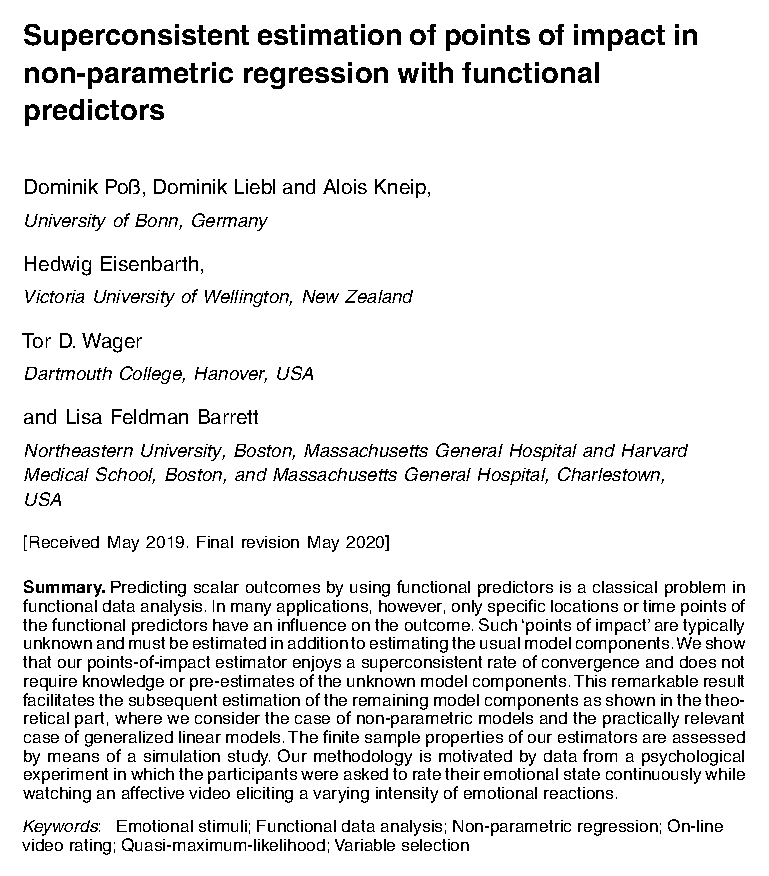
\includegraphics[width=0.45\textwidth]{files/paper-titlepage.pdf}}
\end{figure}
\end{frame}

\begin{frame}{The Setting}{Liebl et al. (2020)}
\begin{figure}[ht]
    \centering
    \vspace{-1cm}
    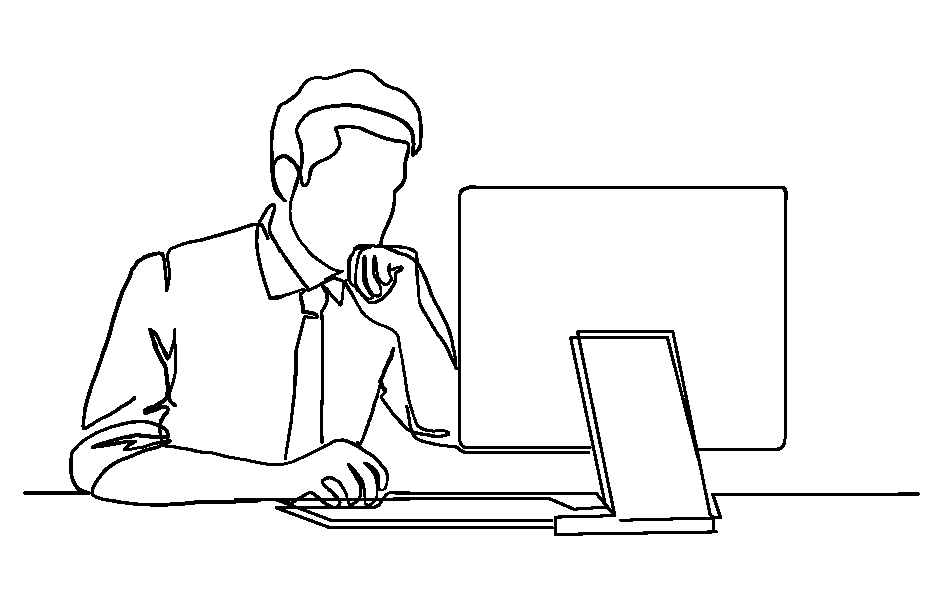
\includegraphics[width=0.55\textwidth]{files/drawing.pdf}
    \fbox{
\includegraphics[width=0.35\textwidth]{files/video-snapshot.pdf}}\\[0.5em]
    \hspace{7.7cm} \footnotesize Figure 1: Snapshot of YouTube video
\end{figure}
\end{frame}

\begin{frame}{The Setting}
    \vspace{-1cm}
    \hspace{0.5cm}
    \begin{centering}
     \begin{tikzpicture}

         % time line
         \draw[line width=0.25mm, ->] (-3.75,0) -- (3.5,0) node [below] {};
         \draw (-3.25, -0.1) -- (-3.25, 0.1) node [below] {\shortstack{\\ \footnotesize Video Start}};
         \draw (2.5, -0.1) -- (2.5, 0.1) node [below] {\shortstack{\\ \footnotesize Video End}};

         % horizontal scale
         \draw[line width=0.25mm] (7, -3) -- (7, 3) node [above] {Sentiment};
         \foreach \x in {-3,-2,...,3}
            \draw (6.8, \x) -- (7.2, \x);

         \node[align=right] at (7.5, 0) {$0$};
         \draw[color=bonnblue, line width=0.3mm] (6.8, 1) -- (7.2, 1);

         % time-point
         \draw[line width=0.3mm, color=bonnblue] (-1, 0.1) -- (-1, -0.1);
         \node[] at (-1, -0.75) {\textcolor{bonnblue}{$\bm{t}$}};
         \draw[color=bonnblue, line width=0.3mm, ->] (-1, 0.25) .. controls (1, 1) and
             (3, 3) .. (5.5, 1) node [right] {\textcolor{bonnblue}{$\bm{X_i(t)}$}};

         \pause
         
         % outcome
         \draw[color=bonngrey, line width=0.3mm, ->] (2.5, -0.5) .. controls (2, -2) and (1.25, -2.2) .. (0, -2.5) node [left] {\textcolor{bonngrey}{$\bm{Y_i} \in \{0, 1\}$}};
         
     \end{tikzpicture}
 \end{centering}
\end{frame}


\newcommand{\brownianmotion}[5]{% points, advance, rand factor, options, end label
\draw[#4] (0,0)
\foreach \x in {1,...,#1}
{   -- ++(#2,rand*#3)
}
node[right] {#5};
}

\begin{frame}{The Data}{Regressors}
\pgfmathsetseed{1341}
\begin{centering}
\begin{tikzpicture}
    \draw[line width=0.25mm, ->] (0, -2) -- (0, 3);
    \draw[line width=0.25mm, ->] (-1, 0) -- (11, 0) node [below] {$t$};
    \brownianmotion{180}{0.05}{0.25}{color=bonngrey, line width=0.2mm}{$X_3(t)$}
    \brownianmotion{180}{0.05}{0.25}{color=bonnyellow, line width=0.2mm}{$X_2(t)$}
    \brownianmotion{180}{0.05}{0.25}{color=bonnblue, line width=0.2mm}{$X_1(t)$}
\end{tikzpicture}
\end{centering}
\end{frame}


\begin{frame}{The Problem}
\pgfmathsetseed{1341}
\vspace{-1cm}
\begin{tikzpicture}[scale=0.8]

    \draw[line width=0.25mm, ->] (0, -2) -- (0, 3);
    \draw[line width=0.25mm, ->] (-1, 0) -- (11, 0) node [below] {$t$};
    \brownianmotion{180}{0.05}{0.25}{color=bonngrey, line width=0.2mm}{$X_3(t)$}
    \brownianmotion{180}{0.05}{0.25}{color=bonnyellow, line width=0.2mm}{$X_2(t)$}
    \brownianmotion{180}{0.05}{0.25}{color=bonnblue, line width=0.2mm}{$X_1(t)$}

    \node[] at (12, 4) {$Y_1 \simeq g\big(X_1(\tau_1), X_1(\tau_2)\big)$};

    \draw[line width=0.2mm, dashed] (2, 4) -- (2, -3) node [right] {$\tau_1$};
    \draw[line width=0.2mm, dashed] (5, 4) -- (5, -3) node [right] {$\tau_2$};

    \node[circle, draw=black, minimum size=1mm, scale=0.9] (c1) at (2, 1.9) {};
    \draw[line width=0.2mm, ->] (c1) .. controls (3, 6) and (10, 6) .. (11.5, 4.5);

    \node[circle, draw=black, minimum size=1mm, scale=0.9] (c2) at (5, 2.6) {};
    \draw[line width=0.2mm, ->] (c2) .. controls (10, 2) and (12.5, 2.5) .. (13, 3.6);

\end{tikzpicture}
\end{frame}


\subsection{The Model}

\begin{frame}{The Model}

    \vspace{-1cm}
    \begin{align*}
        \tcbhighmath[fuzzy halo=1mm with bonnblue,arc=2pt, boxrule=0pt,frame
        hidden]{
            Y_i = g\left(X_i(\tau_1), \dots, X_i(\tau_S) \right) +  \epsilon_i
        }
    \end{align*}

    \vspace{0.5cm}
    \begin{table}[]
    \renewcommand{\arraystretch}{1.5}
        \begin{tabular}{ll}
          \labelitem $X_i = \{ X_i(t) : t \in [0, 1]\}$ & square integrable process\\
          \labelitem $\mathbb{E}\left[\epsilon_i \mid X_i(t) \right] = 0$ &  exogeneity\\
          \labelitem $g : \mathbb{R}^S \to \mathbb{R}$ & \emph{unknown} link function \\
          \labelitem $\tau_1, \dots, \tau_S \in [0, 1]$ &  \emph{unknown} points of impact
        \end{tabular}
    \end{table}

\end{frame}


\begin{frame}{Approach}

    \begin{table}[]
    \renewcommand{\arraystretch}{1.5}
        \begin{tabular}{ll}

        \textcolor{bonnblue}{$1$. stage} & Estimate $S$ and $\tau_1, \dots, \tau_S$\\
        \textcolor{bonnblue}{$2$. stage} & Estimate link function $g$

        \end{tabular}
    \end{table}

    \vspace{1cm}
    \emph{Focus here:} 1. stage

\end{frame}

\section{Review}
\label{section:review}

In this section I present the general setting of \cite{Kneip2020}, albeit restricted to
the definitions, assumptions and theorems that are needed to understand the extension in
section \ref{section:extension}. We assume there is an independent and identically
distributed sample of data $(X_i, y_i)$ for $i=1,\dots,n$ individuals. The functional
regressors $X_i = \{ X_i(t) : t \in [a, b] \}$ is assumed to be a square-integrable
process and $y_i$ is a real-valued random variable. The relationship between regressors
and outcome is modeled as

\[
    y_i = g \left( X_i(\tau_1), \dots, X_i(\tau_S) \right) + \epsilon_i \,,
\]

with $\epsilon_i$ representing the error term satisfying $\expectation{\epsilon_i \mid
X_i(t)} = 0$ for all $t \in [a, b]$. The points of impact are denoted by $\tau_1, \dots,
\tau_S$; where the specific locations $\tau_s \in [a, b]$ are assumed to be unknown a
priori, as well as the number of points $S \in \mathbb{N}_0$. In the same way the link
function $g$ is assumed to be unknown as well. The paper considers centred random
functions $X_i$.

Now one may question how it is possible to estimate the locations as well as their
number while allowing the link function $g$ to be flexible. The upcoming repetitions of
the main assumptions and theorems in \cite{Kneip2020} illustrate that restrictions on
$X_i$ through the covariance kernel suffice for the identification and estimation.

Consider first the covariance kernel of the functional regressor. Let $\sigma(t, s) =
\expectation{X_i(t) X_i(s)}$ denote the covariance kernel of $X_i$.


\begin{assumption}
    Given the kernel $\sigma$, there exists open $\Omega \subset [0, 1]^3$ and twice
    continuously differentiable function $\omega : \Omega \to \mathbb{R}$, as well as
    some $\kappa \in (0, 2)$, such that $\forall s, t \in [0, 1]$

    \[
        \sigma(s, t) = \omega(s, t, |s-t|^{\kappa}) \,.
    \]

    Moreover, $0 < \inf \left\{ c(t) : t \in [0, 1] \right\}$, where $c(t) =
    -\frac{\partial}{\partial z} \omega(t, t, z)|_{z = 0} \,.$
\label{assumption:1}
\end{assumption}

Assumption \ref{assumption:1} restricts the degree of smoothness at the diagonal using
the parameter $\kappa$. This in turn implies certain behavior of the sample paths of the
process. Values with $\kappa < 2$ suggest non-smooth trajectories, while processes with
smooth sample paths and twice continuously differentiable kernel will satisfy the
assumption with $\kappa = 2$. That is, in the current form assumption \ref{assumption:1}
implies that the sample paths of the regressors $X_i$ need to be somewhat rough. Many
known processes fulfill assumption \ref{assumption:1}, for example, Brownian Motion
fulfills it with $\kappa = 1$. In section \ref{section:extension} I present an extension
to this assumption with $\kappa > 2$, allowing for a greater number of processes to be
modeled.


The ability to identify and estimate the points-of-impact relies heavily on the
decomposition presented in theorem \ref{theorem:1}.


\begin{theorem}
Let $X_i$ be a Gaussian process and $g : \mathbb{R}^S \to \mathbb{R}$ an arbitrary
function with continuous partial derivatives almost everywhere. For $s=1,\dots,S$ define

\[
    \vartheta_s = \expectation{\frac{\partial}{\partial x_s} g(X_i(\tau_1), \dots,
    X_i(\tau_S))} \,.
\]

If $0 < \left| \vartheta_s \right| < \infty, \forall s=1,\dots,S$, then we may write,
$\forall t \in [a, b]$

\[
    f_{XY}(t) \stackrel{def}{=} \expectation{X_i(t) y_i} = \sum_{s=1}^S \vartheta_s
    \sigma(t, \tau_s) \,.
\]
\label{theorem:1}
\end{theorem}


Let us henceforth call $f_{XY}$ the cross-covariance (between $X_i$ and $y_i$). In light
of assumption \ref{assumption:1} we know that the kernel $\sigma$ is \emph{not}
two-times differentiable at the diagonal. But then $f_{XY}$ will not be two-times
differentiable at the points-of-impact $\tau_1, \dots, \tau_S$. As it turns out, this
will be enough to ensure identification of the points-of-impact. To differentiate
between any point ($t \in [a, b]$) and a point-of-impact ($t = \tau_s$ for some $s$) the
paper proposes the measure

\[
    f_{ZY}(t) \stackrel{def}{=} f_{XY}(t) - \frac{1}{2} \left( f_{XY}(t + \delta) +
    f_{XY}(t - \delta) \right) \,,
\]

with hyper-parameter $\delta > 0$. Under our current set of assumptions the function
$f_{ZY}$ will be large in absolute value for $t$ close to a point-of-impact. This allows
for the estimation of the points-of-impact using extremum points of an estimated version
of $|f_{ZY}|$. But what is $f_{ZY}$ actually measuring? Notice that the second-order
finite difference of $f_{XY}$ is given by

\begin{align*}
    FD(f_{XY}, \delta, 2)(x) &= \left( f(x + \delta) + f(x - \delta) \right) - 2 f(x)\\
                             &= - \frac{1}{2} f_{ZY}(x) \,,
\end{align*}

where $FD(h, \delta, \ell, x)$ denotes the $\ell$-th order finite difference of function
$h$ with step length $\delta$, evaluated at $x$. Since the criterion function is in
absolute value we can see that using $f_{ZY}$ is proportional to second-order finite
difference of $f_{XY}$. This should make sense, as assumption \ref{assumption:1} implied
that $f_{XY}$ should not be two-times differentiable at the points-of-impact. In that
case, the second-order finite difference formula is expected to be larger at the
points-of-impact than at the other time points.


With this new interpreation in mind we may ask whether we can exploite higher-order
finite differences to relax the assumption on the covariance kernel? The answer is
affirmative and the details will be the concern of section \ref{section:extension}.


At last I state the original version of the estimation algorithm as a comparison to the
more general version supplied in the next section. For the estimation stage we suppose
that the functional regressors $X_i$ are observed at $p$ equidistant points $t_1, \dots,
t_p$ with $t_1 = a, t_p = b$. Since the functions $f_{XY}$ and $f_{ZY}$ are simple
functions of expectations, they can be easily estimated by the standard sample
counterpart, which we denote by $\hat{f}_{XY}$ and $\hat{f}_{ZY}$. The orignal algorithm
is listed as algorithm \ref{algorithm:1}.

\begin{tcolorbox}[standard jigsaw, opacityback=0]

\begin{algorithm}[H]
\caption{Original algorithm from \cite{Kneip2020}, adapted for readability.}
\label{algorithm:1}
\begin{algorithmic}[1]
  \State compute $\hat{f}_{XY}(t_j) = \sum_i X_i(t_j) Y_i / n$, for all $j=1,\dots,p$
  \State choose $\delta > 0$ s.t. $\exists \, k_{\delta} \in \mathbb{N}$ with $1 \leq
  k_{\delta} < (p - 1)/2$ and $\delta = k_{\delta} / (p-1)$
  \State define $\mathcal{J}_{\delta} = \{k_{\delta} + 1, \dots, p - k_{\delta}\}$ and
  set $\ell = 1$
  \State compute $\hat{f}_{ZY}(t_j) = \hat{f}_{XY}(t_j) - (\hat{f}_{XY}(t_j + \delta) +
  \hat{f}_{XY}(t_j - \delta)) / 2$, for all $j \in \mathcal{J}_{\delta}$
  \While{$\mathcal{J}_{\delta} \neq \varnothing$}
  \State estimate $\hat{\tau}_{\ell} = \argmax \left\{|\,\hat{f}_{ZY}(t_j)| : \text{for }
      t_j \text{ with } j \in \mathcal{J}_{\delta}\right\}$
    \State update $\mathcal{J}_{\delta} \leftarrow \mathcal{J}_{\delta} \setminus
    [\hat{\tau}_{\ell} - \sqrt{\delta}, \hat{\tau}_{\ell} + \sqrt{\delta}]$
    \State update $\ell \leftarrow \ell + 1$
  \EndWhile
  \State \textbf{return} $\{\hat{\tau}_{\ell}\}$
\end{algorithmic}
\end{algorithm}

\end{tcolorbox}

\section{Extension}
\label{section:extension}

\textcolor{red}{\lipsum}


\pagestyle{plain}
\pagenumbering{arabic}

\newpage
\nocite{*}
\printbibliography

\appendix


\end{document}
